\documentclass[11pt,a4paper,titlepage]{article}
\usepackage[pdftex]{graphicx}
\usepackage{listings}
\usepackage{titlesec}
\usepackage{float}
\usepackage{enumitem}
\usepackage{color}
\usepackage{pdflscape}
\usepackage{hyperref}
\hypersetup{
	colorlinks,
	citecolor=black,
	filecolor=black,
	linkcolor=black,
	urlcolor=black
}

\setcounter{secnumdepth}{4}

\titleformat{\paragraph}
{\normalfont\normalsize\bfseries}{\theparagraph}{1em}{}
\titlespacing*{\paragraph}
{0pt}{3.25ex plus 1ex minus .2ex}{1.5ex plus .2ex}

\begin{document}
\begin{figure}
	\centering
	
\includegraphics[scale=0.6]{../SE2_IMAGES/Logo_Politecnico_Milano}
\end{figure}
\title{Politecnico di Milano\\A.Y. 2015/2016\\\textbf{Glassfish 4.1}\\Code Inspection\\}
\author{Bernardis Cesare matr. 852509 \and Dagrada Mattia matr.852975}
\date{January 5, 2016}
\maketitle

\newpage

\tableofcontents

\newpage

\section{Checklist}
	\subsection{Naming Conventions}
	\begin{enumerate}
		\item All class names, interface names, method names, class variables, method variables, and constants used should have meaningful names and do what the name suggests.
		\item If one-character variables are used, they are used only for temporary “throwaway” variables, such as those used in for loops.
		\item Class names are nouns, in mixed case, with the first letter of each word in capitalized. Examples: class Raster; class ImageSprite;
		\item Interface names should be capitalized like classes.
		\item Method names should be verbs, with the first letter of each addition word capitalized. Examples: getBackground(); computeTemperature().
		\item Class variables, also called attributes, are mixed case, but might begin with an underscore followed by a lowercase first letter. All the remaining words in the variable name have their first letter capitalized. Examples: \textunderscore windowHeight, timeSeriesData.
		\item Constants are declared using all uppercase with words separated by an underscore. Examples: MIN\textunderscore WIDTH; MAX\textunderscore HEIGHT;
	\end{enumerate}
	\subsection{Indention}
	\begin{enumerate}
		\setcounter{enumi}{7}
		\item Three or four spaces are used for indentation and done so consistently
		\item No tabs are used to indent
	\end{enumerate}
	\subsection{Braces}
	\begin{enumerate}
		\setcounter{enumi}{9}
		\item Consistent bracing style is used, either the preferred “Allman” style (first brace goes underneath the opening block) or the “Kernighan and Ritchie” style (first brace is on the same line of the instruction that opens the new block).
		\item All if, while, do-while, try-catch, and for statements that have only one statement to execute are surrounded by curly braces.
	\end{enumerate}
	\subsection{File Organization}
	\begin{enumerate}
		\setcounter{enumi}{11}
		\item Blank lines and optional comments are used to separate sections (beginning comments, package/import statements, class/interface declarations which include class variable/attributes declarations, constructors, and methods).
		\item Where practical, line length does not exceed 80 characters.
		\item When line length must exceed 80 characters, it does NOT exceed 120 characters.
	\end{enumerate}
	\subsection{Wrapping Lines}
	\begin{enumerate}
		\setcounter{enumi}{14}
		\item Line break occurs after a comma or an operator.
		\item Higher-level breaks are used.
		\item A new statement is aligned with the beginning of the expression at the same level as the previous line.
	\end{enumerate}
	\subsection{Comments}
	\begin{enumerate}
		\setcounter{enumi}{17}
		\item Comments are used to adequately explain what the class, interface, methods, and blocks of code are doing.
		\item Commented out code contains a reason for being commented out and a date it can be removed from the source file if determined it is no longer needed.
	\end{enumerate}
	\subsection{Java Source Files}
	\begin{enumerate}
		\setcounter{enumi}{19}
		\item Each Java source file contains a single public class or interface.
		\item The public class is the first class or interface in the file.
		\item Check that the external program interfaces are implemented consistently with what is described in the javadoc.
		\item Check that the javadoc is complete (i.e., it covers all classes and files part of the set of classes assigned to you).
	\end{enumerate}
	\subsection{Package and Import Statements}
	\begin{enumerate}
		\setcounter{enumi}{23}
		\item If any package statements are needed, they should be the first non-comment statements. Import statements follow.
	\end{enumerate}
	\subsection{Class and Interface Declarations}
	\begin{enumerate}
		\setcounter{enumi}{24}
		\item The class or interface declarations shall be in the following order:
		\begin{enumerate}
			\item class/interface documentation comment
			\item class or interface statement
			\item class/interface implementation comment, if necessary
			\item class (static) variables
			\begin{enumerate}
				\item first public class variables
				\item next protected class variables
				\item next package level (no access modifier)
				\item last private class variables
			\end{enumerate}
			\item instance variables
			\begin{enumerate}
				\item first public instance variables
				\item next protected instance variables
				\item next package level (no access modifier)
				\item last private instance variables
			\end{enumerate}
			\item constructors
			\item methods
		\end{enumerate}
		\item Methods are grouped by functionality rather than by scope or accessibility.
		\item Check that the code is free of duplicates, long methods, big classes, breaking encapsulation, as well as if coupling and cohesion are adequate.
	\end{enumerate}
	\subsection{Initialization and Declarations}
	\begin{enumerate}
		\setcounter{enumi}{27}
		\item Check that variables and class members are of the correct type. Check that they have the right visibility (public/private/protected)
		\item Check that variables are declared in the proper scope
		\item Check that constructors are called when a new object is desired
		\item Check that all object references are initialized before use
		\item Variables are initialized where they are declared, unless dependent upon a computation
		\item Declarations appear at the beginning of blocks (A block is any code surrounded by curly braces “{“ and “}” ). The exception is a variable can be declared in a ‘for’ loop.
	\end{enumerate}
	\subsection{Method Calls}
	\begin{enumerate}
		\setcounter{enumi}{33}
		\item Check that parameters are presented in the correct order
		\item Check that the correct method is being called, or should it be a different method with a similar name
		\item Check that method returned values are used properly
	\end{enumerate}
	\subsection{Arrays}
	\begin{enumerate}
		\setcounter{enumi}{36}
		\item Check that there are no off-by-one errors in array indexing (that is, all required array elements are correctly accessed through the index)
		\item Check that all array (or other collection) indexes have been prevented from going out-of-bounds
		\item Check that constructors are called when a new array item is desired
	\end{enumerate}
	\subsection{Object Comparison}
	\begin{enumerate}
		\setcounter{enumi}{39}
		\item Check that all objects (including Strings) are compared with "equals" and not with "=="
	\end{enumerate}
	\subsection{Output Format}
	\begin{enumerate}
		\setcounter{enumi}{40}
		\item Check that displayed output is free of spelling and grammatical errors
		\item Check that error messages are comprehensive and provide guidance as to how to correct the problem
		\item Check that the output is formatted correctly in terms of line stepping and spacing
	\end{enumerate}
	\subsection{Computation, Comparisons and Assignments}
	\begin{enumerate}
		\setcounter{enumi}{43}
		\item Check that the implementation avoids “brutish programming: (see http://users.csc.calpoly.edu/~jdalbey/SWE/CodeSmells/bonehead.html)
		\item Check order of computation/evaluation, operator precedence and parenthesizing
		\item Check the liberal use of parenthesis is used to avoid operator precedence problems.
		\item Check that all denominators of a division are prevented from being zero
		\item Check that integer arithmetic, especially division, are used appropriately to avoid causing unexpected truncation/rounding
		\item Check that the comparison and Boolean operators are correct
		\item Check throw-catch expressions, and check that the error condition is actually legitimate
		\item Check that the code is free of any implicit type conversions
	\end{enumerate}
	\subsection{Exceptions}
	\begin{enumerate}
		\setcounter{enumi}{51}
		\item Check that the relevant exceptions are caught
		\item Check that the appropriate action are taken for each catch block
	\end{enumerate}
	\subsection{Flow of Control}
	\begin{enumerate}
		\setcounter{enumi}{53}
		\item In a switch statement, check that all cases are addressed by break or return
		\item Check that all switch statements have a default branch
		\item Check that all loops are correctly formed, with the appropriate initialization, increment and termination expressions
	\end{enumerate}
	\subsection{Files}
	\begin{enumerate}
		\setcounter{enumi}{56}
		\item Check that all files are properly declared and opened
		\item Check that all files are closed properly, even in the case of an error
		\item Check that EOF conditions are detected and handled correctly
		\item Check that all file exceptions are caught and dealt with accordingly
	\end{enumerate}
\pagebreak
\section{Classes}
	\subsection{ApplicationHandlers}
		\subsubsection{Details}
		\begin{description}
			\item[Name]: ApplicationHandlers
			\item[Location]: appserver/admingui/common/src/main/java/org/glassfish/admingui/common/handlers
			\item[Package]: org.glassfish.admingui.common.handlers
			\item[Modifiers]: public class
		\end{description}
		\subsubsection{Issues}
		\begin{description}
			\item[18] There are only a few comments in the code of the whole class, not enough,
			given the absence of a proper javadoc.
			\item[23] Javadoc is very poor, it is almost totally missing.
			\item[27] There is a method (getURLs at line 760) that is longer than 50 lines.
		\end{description}
\clearpage
\section{Assigned Class clusters}
	\subsection{Introduction}
	The parts processed in this document belong to the same class ApplicationHandlers.
	In this class the javadoc is almost completely absent and the comments are rare and ineffective.
	The comprehension of the functional roles has been very difficult to deal with, because it has been
	forced to the pure code interpretation. Fortunately a good naming convention has been respected,
	making the understanding a little "less impossible", but yet very superficial.
	\subsection{getLaunchInfo}
		\subsubsection{Description}
		\begin{description}
		\item[Location]: appserver/admingui/common/src/main/java/org/glassfish/admingui/common/handlers/ApplicationHandlers.java
		\item[Name]: getLaunchInfo(String appName, String contextRoot, Map oneRow)
		\item[Modifiers]: private static void
		\item[Start Line]: 368
		\item[Functional Role]: Retrieves some informations about an application (the name of which is passed
		as a parameter). It makes some rest requests and parses the responses to set, in particular, two values
		in the Map passed as parameter: 'contextRoot' (if not passed as parameter) and 'hasLaunch'.
		\end{description}
		\newpage
		\subsubsection{Code}
		\begin{figure}[h!]
			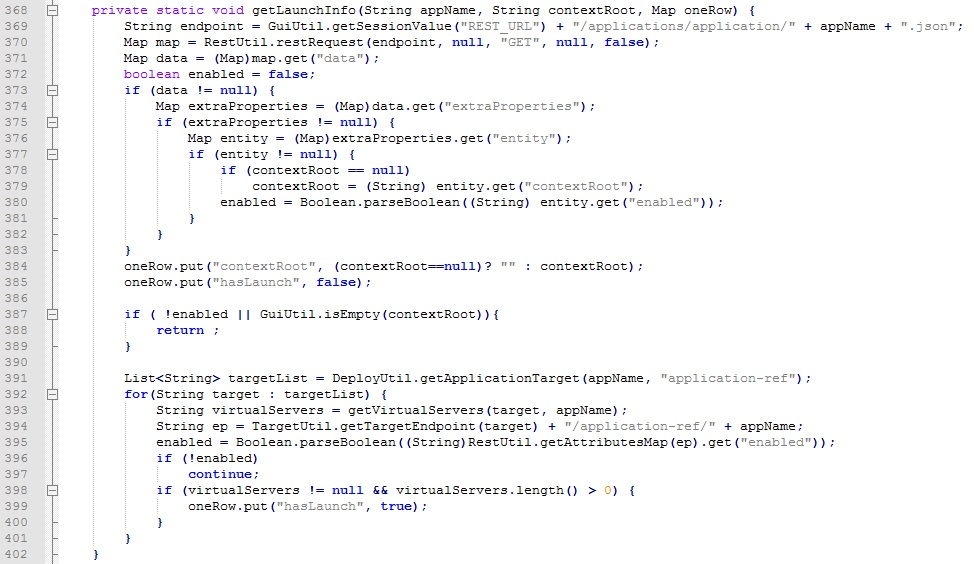
\includegraphics[width=\textwidth]{../SE2_CODE/getlaunchinfo}
		\end{figure}
		\subsubsection{Issues}
		\begin{description}
			\item[11] One statement statements are not surrounded by curly braces
				\begin{itemize}
				\item If at line 378
				\item If at line 396
				\end{itemize}
			\item[13] Multiple lines exceed the 80 characters (spaces included).
				This is not a major issue, because none of them	exceeds the limit of 120 characters on the same line and
				the readability is not compromised.
				\begin{itemize}
					\item Line 369 could be divided into segments after '+' operator.
					\item Line 380
					\item Line 391
					\item Line 394 could be divided into segments after '+' operator.
					\item Line 395
				\end{itemize}
			\item[18] This is a private method, so it is comprehensible that no javadoc has been provided, but
			without comments it is quite hard to understand what the method does.
			\item[33] This will NOT be considered an issue: at line 396 there is a declaration and initialization
			that is not at the beginning of a "physical" block, but it can be considered an initialization
			for the loop at line 397 (in order to make it easier to understand).
			\item[52] There are no exceptions caught or thrown explicitly. There are extra controls to avoid method
			calls on null objects and some other measures to avoid execution errors, but they might not be enough.
		\end{description}
	\clearpage
	\subsection{if(appPropsMap != null)}
		\subsubsection{Description}
		\begin{description}
		\item[Location]: appserver/admingui/common/src/main/java/org/glassfish/admingui/common/handlers/ApplicationHandlers.java
		\item[Name]: if(appPropsMap != null)
		\item[Start Line]: 617
		\item[Functional Role]: For every value in appPropsMap (which is a Map containing, probably,
		the properties of an application) retrieves some informations and puts them into a Map that will be
		added to the result object.
		\end{description}
		\subsubsection{Code}
		\begin{figure}[h!]
			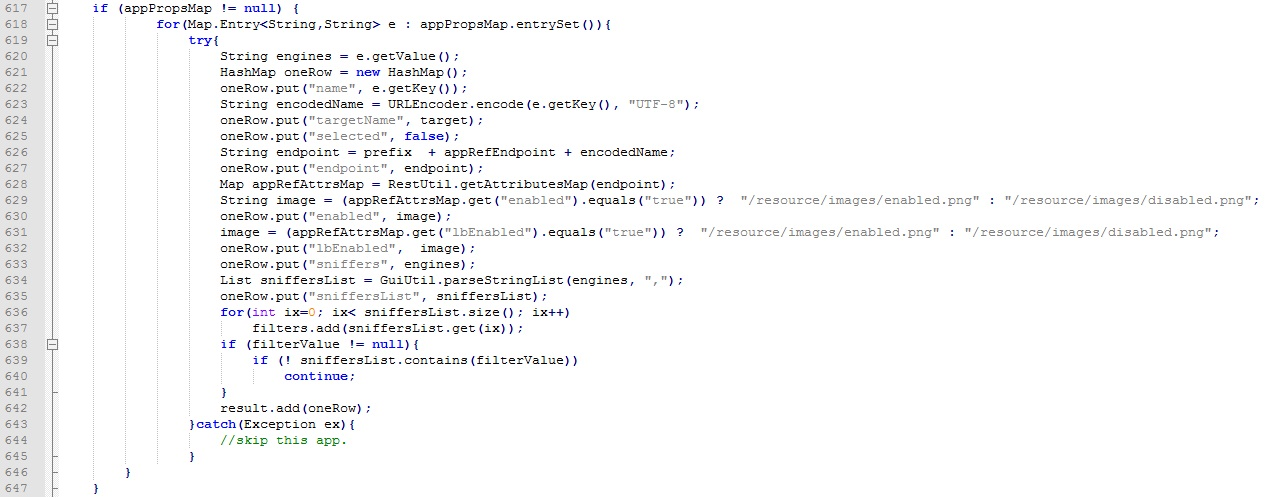
\includegraphics[width=\textwidth]{../SE2_CODE/ifapppropsmap}
		\end{figure}
		\subsubsection{Issues}
		\begin{description}
			\item[9] A tab is used to indent line 617
			\item[11] One statement statements are not surrounded by curly braces
			\begin{itemize}
				\item For at line 636
				\item If at line 639
			\end{itemize}
			\item[14] Two lines exceed the 120 characters (spaces included).
			\begin{itemize}
				\item Line 629 (151 chars) could be divided into '?:' operator segments.
				\item Line 631 (146 chars) could be divided into '?:' operator segments.
			\end{itemize}
			\item[17] There is a mistake in the indentation: the wrapping If is not aligned with the upper statement.
			\item[18] In this piece of code (that is a particular part of a method) there are no sensible comments.
			Unfortunately also the javadoc is incomplete and is not clear the role of this public method.
			\item[23] The javadoc for this method is incomplete, practically it is totally missing.
			\item[33] In the For at line 618 there are several declarations and initializations mixed with "put"
			operations in the output row.
			\item[53] There is a single try-catch block for the whole piece of code. It is not very elegant, but
			it avoids errors. The problem is that the general exception is catched, but no actions are properly taken.
		\end{description}
\section{Additional Material}

\end{document}